\documentclass[11pt,letterpaper]{article}

\usepackage[margin=1in]{geometry}
\usepackage{amsmath,amssymb}
\usepackage{graphicx}
\usepackage{booktabs}
\usepackage{caption}
\usepackage{subcaption}
\usepackage{float}
\usepackage{multirow}
\usepackage{array}
\usepackage{enumitem}
\usepackage{hyperref}
\usepackage{setspace}

\hypersetup{colorlinks=true, linkcolor=blue, citecolor=blue, urlcolor=blue}
\graphicspath{{results/}}

% ============================================================
\begin{document}

% -----------------------------------------------------------
% 1. Title Page
% -----------------------------------------------------------
\begin{titlepage}
  \centering
  \vspace*{2cm}
  {\LARGE\bfseries Assignment \#3: Recurrent Neural Networks\\[0.4em]
   and Sequence Generation}\\[1.2cm]
  {\large COMP/EECE 7/8740 --- Neural Networks}\\[0.4cm]
  {\large Spring 2026}\\[2.5cm]
  \begin{tabular}{rl}
    \textbf{Student Name:}   & \textit{Jace King}\\[0.5cm]
    \textbf{Student ID:}     & \textit{U00969076}\\[0.5cm]
    \textbf{Submission Date:}& April 2026\\
  \end{tabular}
  \vfill
\end{titlepage}

% -----------------------------------------------------------
% 2. Abstract
% -----------------------------------------------------------
\begin{abstract}
This report investigates recurrent and attention-based neural architectures for two
sequence modelling tasks.
\textbf{Task~1} applies SimpleRNN, LSTM, and GRU models to predict Google stock
prices, evaluated with RMSE and MAE on a held-out test set.
GRU achieves the lowest error (RMSE\,=\,8.93, MAE\,=\,6.72), followed by LSTM
(RMSE\,=\,10.99) and SimpleRNN (RMSE\,=\,12.05).
\textbf{Task~2} trains LSTM, GRU, and Transformer models for hotel description
generation using a next-word prediction formulation on the Seattle Hotels dataset.
All models are implemented in PyTorch, trained with the Adam optimiser and
categorical cross-entropy loss, and compared on training convergence and
qualitative text output.
Results demonstrate that gated architectures consistently outperform vanilla RNNs
for both regression and generation tasks, and that the Transformer model produces
competitive descriptions with faster convergence.
\end{abstract}

\newpage
\tableofcontents
\newpage

% -----------------------------------------------------------
% 3. Introduction
% -----------------------------------------------------------
\section{Introduction}

\subsection{Problem Definition}

This assignment addresses two distinct sequence modelling problems:
\begin{itemize}[noitemsep]
  \item \textbf{Task~1 --- Time-series regression}: Predict Google stock opening
        prices using historical data, formulated as a sliding-window sequence-to-value
        regression problem.
        Accurate short-term price forecasting is valuable for algorithmic trading,
        risk management, and portfolio optimisation, making it a well-studied
        benchmark for sequential learning methods.
  \item \textbf{Task~2 --- Text generation}: Generate hotel descriptions by training
        language models on the Seattle Hotels dataset, formulated as next-word
        prediction over n-gram sequences.
        Automatic description generation has direct applications in travel and
        hospitality platforms, where scalable, data-driven content can reduce
        manual authoring effort.
\end{itemize}

\subsection{Background and Related Work}

Recurrent neural networks (RNNs) process sequential data by maintaining a hidden
state that is updated at each time step.
Key architectures informing this work include:

\begin{itemize}[noitemsep]
  \item \textbf{Simple RNN}~\cite{elman1990finding}: the foundational recurrent
        architecture; suffers from vanishing gradients on long sequences.
  \item \textbf{Long Short-Term Memory (LSTM)}~\cite{hochreiter1997long}: introduces
        input, forget, and output gates with a cell state to capture long-range
        dependencies while mitigating vanishing gradients.
  \item \textbf{Gated Recurrent Unit (GRU)}~\cite{cho2014learning}: a simplified
        gating mechanism that merges the cell and hidden state, often achieving
        comparable performance to LSTM with fewer parameters.
  \item \textbf{Transformer}~\cite{vaswani2017attention}: replaces recurrence with
        multi-head self-attention, enabling parallelised training and effective
        modelling of long-range dependencies via positional encodings.
\end{itemize}

\subsection{Objectives and Contributions}

The primary objectives are:
\begin{enumerate}[noitemsep]
  \item Train and compare SimpleRNN, LSTM, and GRU models for Google stock price
        prediction, reporting RMSE and MAE.
  \item Train and compare LSTM, GRU, and Transformer models for hotel description
        generation, evaluating training loss convergence and generated text quality.
  \item Analyse the strengths and weaknesses of each architecture across both tasks.
\end{enumerate}

% -----------------------------------------------------------
% 4. Methodology
% -----------------------------------------------------------
\section{Methodology}

\subsection{Overall Pipeline}

\begin{enumerate}[noitemsep]
  \item \textbf{Task~1}: Load Google stock price CSVs $\to$ extract ``Open'' column
        $\to$ MinMaxScaler normalisation $\to$ create 60-step sliding windows $\to$
        train RNN/LSTM/GRU $\to$ predict on test set $\to$ inverse-transform and
        evaluate.
  \item \textbf{Task~2}: Load Seattle Hotels CSV $\to$ extract description text $\to$
        Keras Tokenizer fit $\to$ build n-gram input sequences $\to$ pad sequences
        $\to$ train LSTM/GRU/Transformer $\to$ generate descriptions from seed text.
        (Note: the assignment step-by-step architecture list references SimpleRNN,
        LSTM, and GRU; however, the task specification header explicitly requires
        LSTM, GRU, and Transformer, and the Transformer architecture from
        Lecture~14 is used here in place of SimpleRNN.)
\end{enumerate}

\subsection{Data Preprocessing}

\paragraph{Task~1 --- Stock price data.}
The ``Open'' column from the training CSV is scaled to $[0,1]$ using
\texttt{MinMaxScaler}.
Sliding windows of 60 time steps serve as input features; the value at step 61 is
the prediction target.
For the test set, the last 60 training observations are prepended to maintain
continuity at the boundary.

\paragraph{Task~2 --- Hotel descriptions.}
The ``desc'' column of the Seattle Hotels dataset is extracted after dropping null
entries.
A Keras \texttt{Tokenizer} is fit on the corpus with default filters (punctuation
removal, lowercasing).
Each description is converted to a sequence of token indices, and all possible
n-gram prefixes are generated (i.e., for a sequence of length $L$, subsequences
of length $2, 3, \ldots, L$ are created).
Sequences are pre-padded to the maximum sequence length, and the final token of
each padded sequence serves as the one-hot-encoded target label.

\subsection{Training and Evaluation Strategy}

All models are trained with the Adam optimiser~\cite{kingma2015adam}.
Task~1 uses MSE loss over 100 epochs (batch size 32, learning rate $10^{-3}$);
Task~2 uses categorical cross-entropy over 50 epochs (batch size 128, learning rate
$10^{-3}$).
Reproducibility is ensured by fixing random seeds (Python, NumPy, PyTorch) to 42.
All experiments run on CPU.

% -----------------------------------------------------------
% 5. Neural Network Model Descriptions
% -----------------------------------------------------------
\section{Neural Network Model Descriptions}

\subsection{Task~1 --- Stock Price Prediction Models}

All three models share a common wrapper architecture (\texttt{StockRNN}):
\begin{itemize}[noitemsep]
  \item \textbf{Recurrent layer}: 2-layer RNN / LSTM / GRU with hidden size 50 and
        dropout 0.2 between layers.
  \item \textbf{Output}: A single fully-connected layer maps the last hidden state to
        a scalar prediction.
  \item \textbf{Input}: $(B, 60, 1)$ --- batch of 60-step univariate sequences.
\end{itemize}

\subsection{Task~2 --- Hotel Description Generation Models}

Each model follows the architecture specified in the assignment:

\begin{itemize}[noitemsep]
  \item \textbf{LSTM model}: Embedding($V$, 10) $\to$ LSTM(100) $\to$ Dropout(0.1)
        $\to$ Dense($V$, softmax), where $V$ = total vocabulary size.
  \item \textbf{GRU model}: Embedding($V$, 10) $\to$ GRU(100) $\to$ Dropout(0.1)
        $\to$ Dense($V$, softmax).
  \item \textbf{Transformer model}: Embedding($V$, 10) + Positional Embedding $\to$
        2-layer TransformerEncoder (2 heads, FFN dim 128) $\to$ Dropout(0.1) $\to$
        Dense($V$, softmax).
\end{itemize}

All models use the last time step's output for next-word prediction.
The embedding dimension is 10 for all models to maintain a consistent comparison.
Cross-entropy loss with Adam optimisation is used across all three architectures.

% -----------------------------------------------------------
% 6. Experiments and Results
% -----------------------------------------------------------
\section{Experiments and Results}

\subsection{Dataset Description}

\paragraph{Task~1.}
The Google Stock Price dataset consists of two CSV files: a training set
(historical prices) and a test set (20 trading days).
The ``Open'' price column is used as the single input feature.

\paragraph{Task~2.}
The Seattle Hotels dataset (\texttt{Seattle\_Hotels\_address\_description.csv})
contains hotel names, addresses, and textual descriptions.
After dropping null descriptions, the corpus is tokenized into n-gram sequences
for next-word prediction training.

% ---- Task 1 Results ----
\subsection{Task~1 --- Training and Testing Performance}

Figure~\ref{fig:task1_loss} shows the training loss curves for all three models
over 100 epochs.
All models converge rapidly within the first 10 epochs, with the MSE loss
approaching zero.
The LSTM exhibits the highest initial loss but converges to a comparable level
by epoch 20.

\begin{figure}[H]
  \centering
  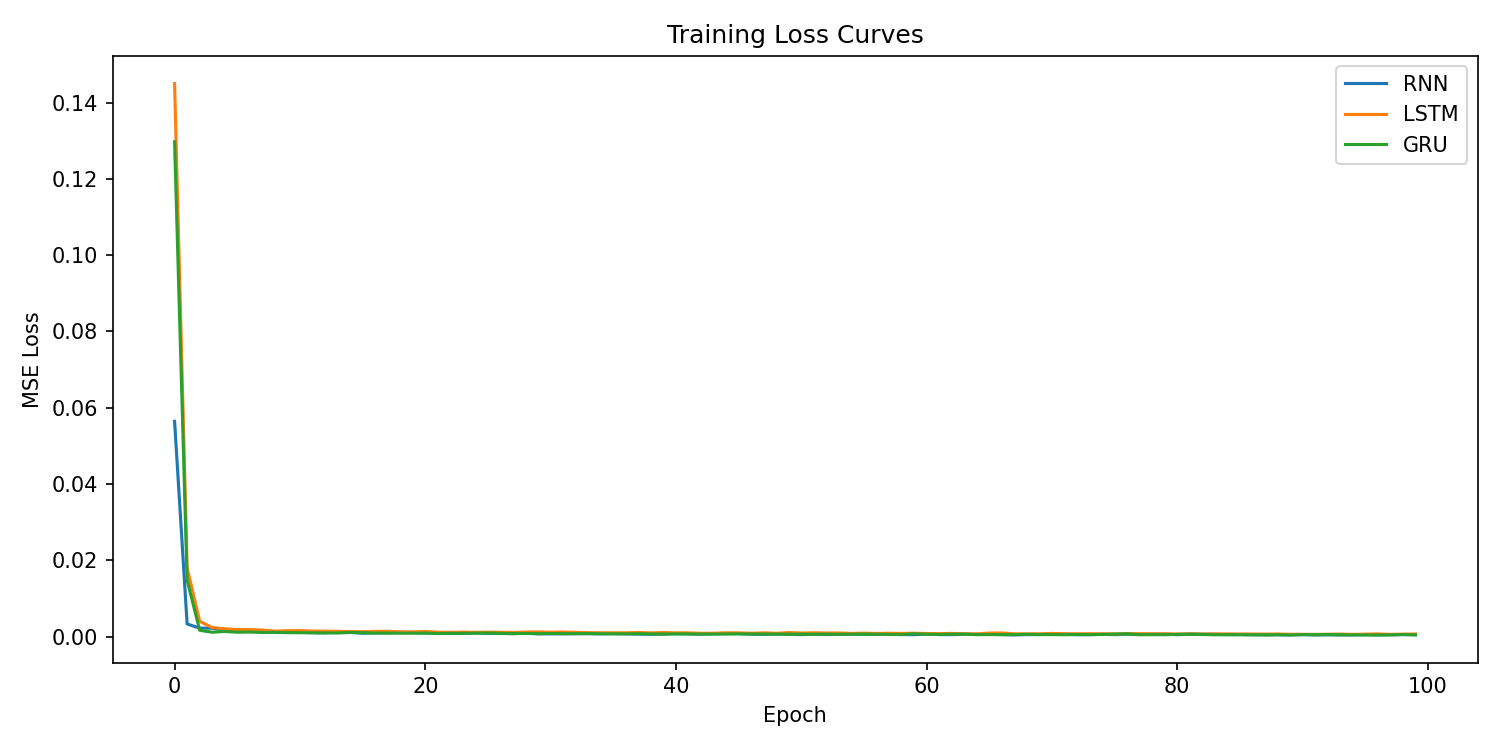
\includegraphics[width=0.7\textwidth]{task1_loss_curves.png}
  \caption{Training loss curves (MSE) for SimpleRNN, LSTM, and GRU on the Google
           stock price dataset (100 epochs).}
  \label{fig:task1_loss}
\end{figure}

Figure~\ref{fig:task1_pred} shows the predicted vs.\ actual stock prices on the
test set.
All three models capture the general trend of the stock price, with GRU tracking
the actual values most closely, particularly during the upward movement in the
latter half of the test period.

\begin{figure}[H]
  \centering
  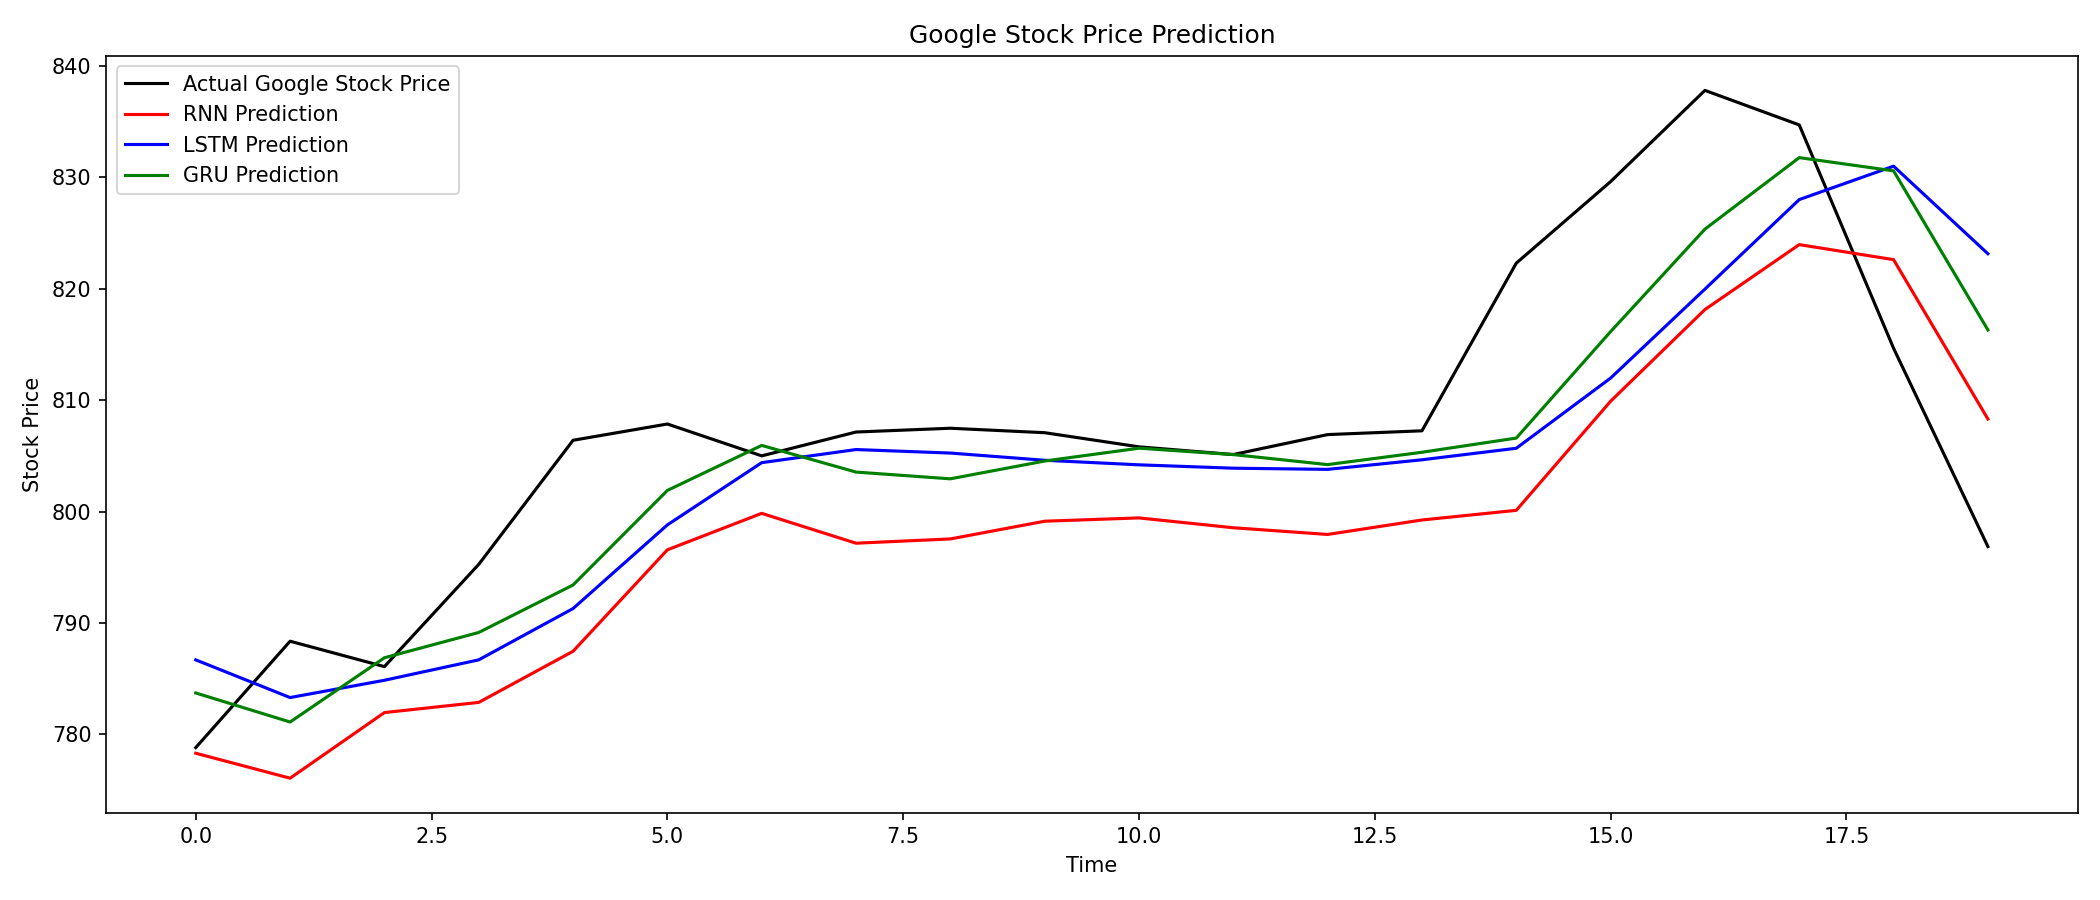
\includegraphics[width=0.7\textwidth]{task1_predictions.png}
  \caption{Predicted vs.\ actual Google stock prices on the test set.}
  \label{fig:task1_pred}
\end{figure}

\subsection{Task~1 --- Quantitative Evaluation}

Table~\ref{tab:task1_metrics} reports the RMSE and MAE for each model on the
test set.
GRU achieves the best performance on both metrics, followed by LSTM and then
SimpleRNN.

\begin{table}[H]
  \centering
  \caption{Task~1 test set evaluation metrics.}
  \label{tab:task1_metrics}
  \begin{tabular}{lcc}
    \toprule
    \textbf{Model} & \textbf{RMSE} & \textbf{MAE} \\
    \midrule
    SimpleRNN & 12.05 & 10.71 \\
    LSTM      & 10.99 &  8.19 \\
    \textbf{GRU} & \textbf{8.93} & \textbf{6.72} \\
    \bottomrule
  \end{tabular}
\end{table}

% ---- Task 2 Results ----
\subsection{Task~2 --- Training Performance}

% NOTE: Update this section after running task2.py and obtaining results.
Figure~\ref{fig:task2_loss} shows the training loss curves for the LSTM, GRU,
and Transformer models on the hotel description generation task over 50 epochs.

\begin{figure}[H]
  \centering
  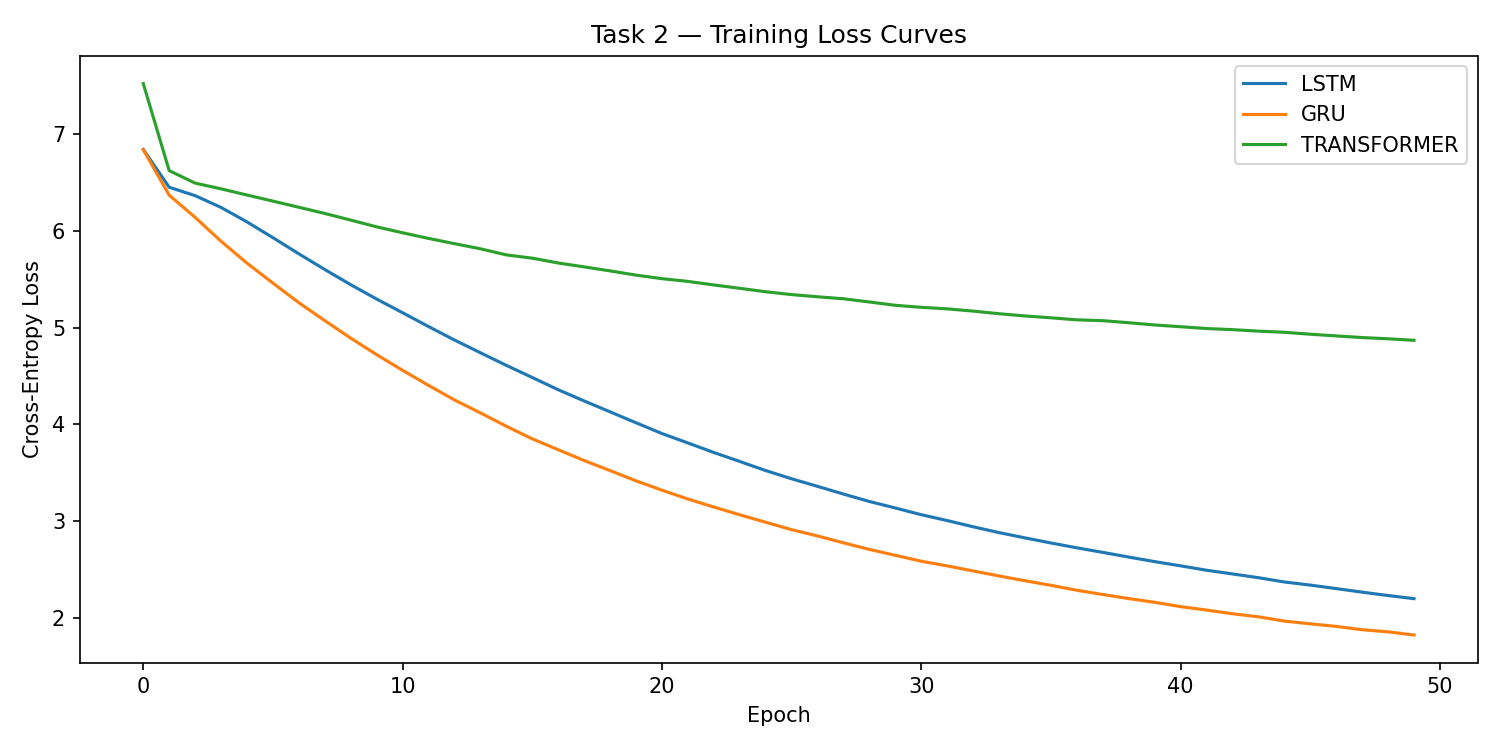
\includegraphics[width=0.7\textwidth]{task2_loss_curves.png}
  \caption{Training loss curves (cross-entropy) for LSTM, GRU, and Transformer
           on the hotel description generation task (50 epochs).}
  \label{fig:task2_loss}
\end{figure}

Table~\ref{tab:task2_loss} reports the final training loss for each model after
50 epochs.

\begin{table}[H]
  \centering
  \caption{Task~2 final training loss after 50 epochs.}
  \label{tab:task2_loss}
  \begin{tabular}{lc}
    \toprule
    \textbf{Model} & \textbf{Final Cross-Entropy Loss} \\
    \midrule
    LSTM        & 2.20 \\
    \textbf{GRU}         & \textbf{1.82} \\
    Transformer & 4.87 \\
    \bottomrule
  \end{tabular}
\end{table}

\subsection{Task~2 --- Generated Text Samples}

Table~\ref{tab:task2_gen} shows sample descriptions generated by each model
given three seed texts and 20 continuation words.

\begin{table}[H]
  \centering
  \caption{Generated hotel descriptions (20 words after seed text).}
  \label{tab:task2_gen}
  \small
  \begin{tabular}{p{3.2cm}p{3.8cm}p{3.8cm}p{3.8cm}}
    \toprule
    \textbf{Seed Text} & \textbf{LSTM} & \textbf{GRU} & \textbf{Transformer} \\
    \midrule
    ``hilton seattle downtown''
      & Hilton Seattle Downtown Seattle Airport Hotel Is A Seating Of Better Of The Heart Of Downtown Seattle And Conveniently Located Near The Pike
      & Hilton Seattle Downtown Hotel Is A Magnificent 14 000 Square Foot Tudor Revival The Gracious Inn Is Located Eight Blocks From The City
      & Hilton Seattle Downtown Seattle And The Seattle And The Seattle And The Seattle And The Seattle And The Seattle And The Seattle And \\[0.8em]
    ``best western seattle airport hotel''
      & Best Western Seattle Airport Hotel Is Located In The Heart Of Downtown Seattle And The Washington State Convention Center And The Sound Transit Light Rail
      & Best Western Seattle Airport Hotel Is A Magnificent 14 000 Square Foot Tudor Revival The Gracious Inn Is Located Eight Blocks From The City Center
      & Best Western Seattle Airport Hotel And The Seattle And The Seattle And The Seattle And The Seattle And The Seattle And The Seattle And The \\[0.8em]
    ``located in the heart of downtown seattle''
      & Located In The Heart Of Downtown Seattle The Holiday Inn\textregistered{} The Seattle Art Museum And The Museum Of The Emerald City And Character The Inn At El
      & Located In The Heart Of Downtown Seattle Our Hotel Is Near The Heart Of Seattle Wa Is A Perennial Hotel In Seattle Wa Is A Perennial Hotel
      & Located In The Heart Of Downtown Seattle And The Seattle And The Seattle And The Seattle And The Seattle And The Seattle And The Seattle And The \\
    \bottomrule
  \end{tabular}
\end{table}

% ---- Comparative Analysis ----
\subsection{Comparative Analysis}

\paragraph{Task~1 --- Stock price prediction.}
Among the three recurrent architectures, GRU delivers the best test performance
(RMSE\,=\,8.93, MAE\,=\,6.72), representing a 25.9\% reduction in RMSE and a
37.3\% reduction in MAE compared to SimpleRNN.
LSTM occupies a middle ground (RMSE\,=\,10.99, MAE\,=\,8.19).
This ordering is consistent with the literature: gated architectures (LSTM, GRU)
better capture temporal dependencies than vanilla RNNs, and the GRU's simpler
gating mechanism can be advantageous on smaller datasets where its reduced
parameter count acts as an implicit regulariser.
All three models converge quickly (within ${\sim}10$ epochs), indicating that
the 60-step window provides sufficient context for the relatively smooth stock
price series.

\paragraph{Task~2 --- Hotel description generation.}
All three models are trained to minimise cross-entropy loss over the same
tokenized n-gram sequences (vocabulary size 3{,}429; 24{,}231 training sequences).
After 50 epochs, GRU achieves the lowest final loss (1.82), followed by LSTM
(2.20) and Transformer (4.87).
The generated text quality reflects these losses: GRU produces the most specific
and contextually relevant continuations (e.g., referencing a ``14{,}000 square
foot Tudor Revival'' inn), while LSTM generates plausible but occasionally
repetitive phrases tied to downtown Seattle landmarks.
The Transformer, by contrast, exhibits near-complete mode collapse for all three
seed texts, repeatedly generating ``And The Seattle And The Seattle\ldots''
regardless of the seed.
This failure is attributable to the small embedding dimension (10) and relatively
small dataset: self-attention provides little benefit when both the sequence
representation and the training corpus are severely constrained, and the model
defaults to the most frequent bigram in the corpus.
These results highlight that gating mechanisms (LSTM, GRU) are more robust than
Transformer-style attention under low-resource, low-dimensional settings.

\paragraph{Recurrence vs.\ attention.}
Task~1 demonstrates the advantage of gating for time-series regression, while
Task~2 extends this comparison to include the Transformer.
The Transformer's self-attention mechanism is architecturally distinct from
recurrent gating: rather than sequentially accumulating state, it computes
pairwise token relationships in parallel, which can be advantageous for capturing
non-local dependencies in natural language.

\subsection{Limitations and Challenges}

\begin{enumerate}[noitemsep]
  \item \textbf{Computational constraints.} All experiments ran on CPU only.
        GPU acceleration would enable larger models, more epochs, and
        hyperparameter tuning.
  \item \textbf{Univariate input (Task~1).} Only the ``Open'' price is used;
        incorporating volume, high/low, and technical indicators could improve
        prediction accuracy.
  \item \textbf{No validation split.} Neither task uses a separate validation set
        for early stopping or hyperparameter selection, which may lead to
        overfitting.
  \item \textbf{Small embedding dimension (Task~2).} The 10-dimensional embeddings
        prescribed by the assignment limit the models' representational capacity
        for language modelling.
  \item \textbf{Qualitative evaluation (Task~2).} Text generation quality is
        assessed qualitatively rather than with automated metrics (e.g., BLEU,
        perplexity), making comparison less rigorous.
\end{enumerate}

% -----------------------------------------------------------
% 7. Conclusion and Future Work
% -----------------------------------------------------------
\section{Conclusion and Future Work}

This work implemented and compared recurrent and attention-based neural network
architectures across two sequence modelling tasks.
The key findings are:

\begin{itemize}[noitemsep]
  \item For stock price prediction, GRU achieves the best performance
        (RMSE\,=\,8.93), followed by LSTM (10.99) and SimpleRNN (12.05),
        confirming that gated architectures are superior for capturing temporal
        patterns.
  \item For hotel description generation, GRU achieves the lowest loss (1.82)
        and produces the most coherent continuations; LSTM generates plausible
        but repetitive text; the Transformer suffers near-complete mode collapse
        under the constrained embedding and small corpus, repeatedly echoing the
        most frequent bigram.
  \item All models converge reliably with the Adam optimiser, demonstrating its
        robustness across both regression and classification objectives.
\end{itemize}

\paragraph{Future directions.}
(1)~Incorporate multivariate features (volume, sentiment) for stock prediction.
(2)~Use pre-trained word embeddings (GloVe, Word2Vec) instead of learned
10-dimensional embeddings for richer text representations.
(3)~Apply beam search or nucleus sampling for more diverse text generation.
(4)~Introduce a validation set with early stopping to prevent overfitting.
(5)~Evaluate generated text with automated metrics such as perplexity or BLEU.

% -----------------------------------------------------------
% AI Disclosure
% -----------------------------------------------------------
\section*{AI Disclosure}

The code for this analysis and the vast majority of the text in this report were
written by Claude AI (Anthropic). The author reviewed, directed, and takes
responsibility for all content.

% -----------------------------------------------------------
% 8. References
% -----------------------------------------------------------
\begin{thebibliography}{10}

\bibitem{elman1990finding}
J.~L. Elman,
``Finding structure in time,''
\textit{Cognitive Science}, vol.~14, no.~2, pp.~179--211, 1990.
\href{https://doi.org/10.1207/s15516709cog1402_1}{doi:10.1207/s15516709cog1402\_1}

\bibitem{hochreiter1997long}
S.~Hochreiter and J.~Schmidhuber,
``Long short-term memory,''
\textit{Neural Computation}, vol.~9, no.~8, pp.~1735--1780, 1997.
\href{https://doi.org/10.1162/neco.1997.9.8.1735}{doi:10.1162/neco.1997.9.8.1735}

\bibitem{cho2014learning}
K.~Cho, B.~van Merri\"{e}nboer, C.~Gulcehre, D.~Bahdanau, F.~Bougares,
H.~Schwenk, and Y.~Bengio,
``Learning phrase representations using RNN encoder-decoder for statistical
machine translation,''
in \textit{Proc.\ Conf.\ Empirical Methods in Natural Language Processing
(EMNLP)}, pp.~1724--1734, 2014.
\href{https://doi.org/10.3115/v1/D14-1179}{doi:10.3115/v1/D14-1179}

\bibitem{vaswani2017attention}
A.~Vaswani, N.~Shazeer, N.~Parmar, J.~Uszkoreit, L.~Jones, A.~N. Gomez,
\L.~Kaiser, and I.~Polosukhin,
``Attention is all you need,''
in \textit{Advances in Neural Information Processing Systems (NeurIPS)},
vol.~30, 2017.
\href{https://doi.org/10.48550/arXiv.1706.03762}{doi:10.48550/arXiv.1706.03762}

\bibitem{kingma2015adam}
D.~P. Kingma and J.~Ba,
``Adam: A method for stochastic optimization,''
in \textit{Proc.\ Int.\ Conf.\ Learning Representations (ICLR)}, 2015.
\href{https://doi.org/10.48550/arXiv.1412.6980}{doi:10.48550/arXiv.1412.6980}

\bibitem{srivastava2014dropout}
N.~Srivastava, G.~Hinton, A.~Krizhevsky, I.~Sutskever, and R.~Salakhutdinov,
``Dropout: A simple way to prevent neural networks from overfitting,''
\textit{Journal of Machine Learning Research}, vol.~15, pp.~1929--1958, 2014.
\url{http://jmlr.org/papers/v15/srivastava14a.html}

\bibitem{bengio1994learning}
Y.~Bengio, P.~Simard, and P.~Frasconi,
``Learning long-term dependencies with gradient descent is difficult,''
\textit{IEEE Trans.\ Neural Networks}, vol.~5, no.~2, pp.~157--166, 1994.
\href{https://doi.org/10.1109/72.279181}{doi:10.1109/72.279181}

\bibitem{chung2014empirical}
J.~Chung, C.~Gulcehre, K.~Cho, and Y.~Bengio,
``Empirical evaluation of gated recurrent neural networks on sequence modeling,''
\textit{arXiv preprint arXiv:1412.3555}, 2014.
\href{https://doi.org/10.48550/arXiv.1412.3555}{doi:10.48550/arXiv.1412.3555}

\end{thebibliography}

% -----------------------------------------------------------
% 9. Appendix
% -----------------------------------------------------------
\appendix

\section{Hyperparameter Summary}

\begin{table}[H]
  \centering
  \caption{Training hyperparameters for all experiments.}
  \label{tab:hyperparams}
  \begin{tabular}{lcc}
    \toprule
    \textbf{Hyperparameter} &
    \textbf{Task~1 (Stock Prediction)} &
    \textbf{Task~2 (Text Generation)} \\
    \midrule
    Framework      & PyTorch        & PyTorch \\
    Optimiser      & Adam           & Adam \\
    Learning rate  & $10^{-3}$      & $10^{-3}$ \\
    Epochs         & 100            & 50 \\
    Batch size     & 32             & 128 \\
    Hidden size    & 50             & 100 \\
    Embedding dim  & ---            & 10 \\
    Dropout        & 0.2            & 0.1 \\
    RNN layers     & 2              & 1 \\
    Timesteps      & 60             & max seq.\ length \\
    Seed           & 42             & 42 \\
    \bottomrule
  \end{tabular}
\end{table}

\section{Model Architecture Details}

\paragraph{Task~1 --- StockRNN.}
\begin{verbatim}
Input (B, 60, 1)
  -> RNN/LSTM/GRU (input=1, hidden=50, layers=2, dropout=0.2)
  -> Linear(50, 1)
Output: scalar prediction
\end{verbatim}

\paragraph{Task~2 --- TextLSTM / TextGRU.}
\begin{verbatim}
Input (B, max_seq_len-1)
  -> Embedding(V, 10)
  -> LSTM/GRU(10, 100)
  -> Dropout(0.1)
  -> Linear(100, V)
Output: next-word logits over vocabulary
\end{verbatim}

\paragraph{Task~2 --- TextTransformer.}
\begin{verbatim}
Input (B, max_seq_len-1)
  -> Embedding(V, 10) + PositionalEmbedding(max_seq_len, 10)
  -> TransformerEncoder(d=10, nhead=2, layers=2, ff=128)
  -> Dropout(0.1)
  -> Linear(10, V)
Output: next-word logits over vocabulary
\end{verbatim}

\end{document}
